% !TeX root = ../build/main.tex

\subsection{Voter circuit}

Figure~\ref{fig:circuit-voter}.

\begin{figure}[H]
	\centerline{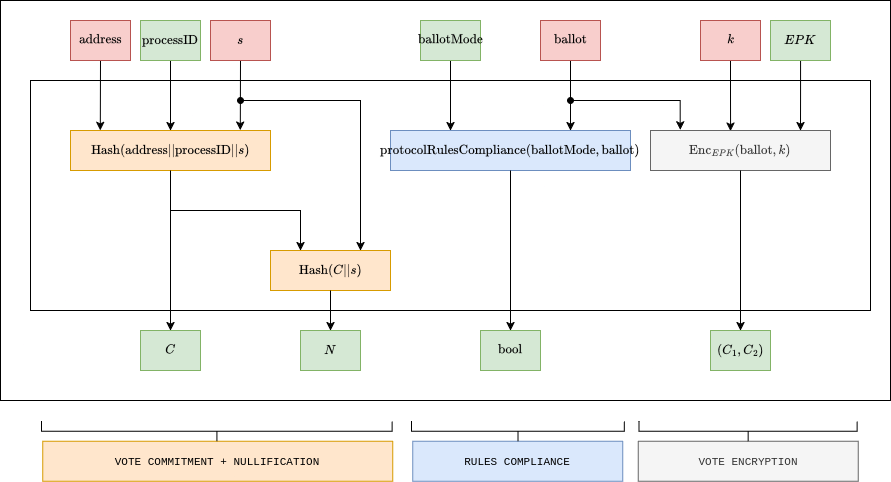
\includegraphics[width=400pt,draft=false]{\figs/circuit-voter}}
	\caption{Voter circuit. All public values are framed in green.}
	\label{fig:circuit-voter}
\end{figure}

\textbf{Inputs}:

\begin{itemize}
	\setlength\itemsep{1em}
		\item \public $\processid$: process identifier.
		\item \public $\ballotmode$: ballot protocol configuration.
		\item \public $EPK$: encryption public key.
		\item \public voter's weight.
		\item \public $C$: commitment.
		\item \public $N$: nullifier.
		\item \public $(C_1, C_2)$: encrypted ballot.
%
		\item \private $\address$: voter's address.
		\item \private $ballot$: plaintext voter's voting choice.
		\item \private $s$: blinder factor (secret).
		\item \private $k$: random scalar.
\end{itemize}


\newpage
\subsection{Authentication circuit}

Figure~\ref{fig:circuit-authentication}.

\begin{figure}[H]
	\centerline{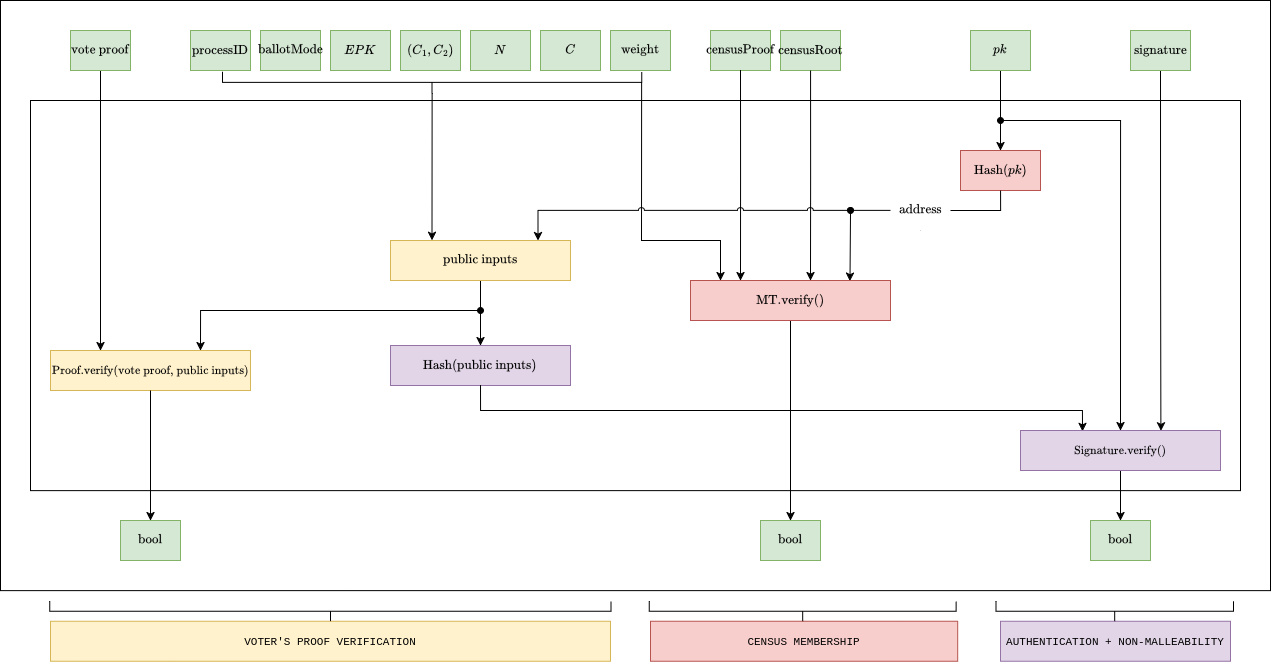
\includegraphics[width=400pt,draft=false]{\figs/circuit-authentication}}
	\caption{Authentication circuit. All public values are framed in green.}
	\label{fig:circuit-authentication}
\end{figure}

\textbf{Inputs}:

\begin{itemize}
	\setlength\itemsep{1em}
		\item \public $\text{voteProof}$: voter's proof.
		\item \public $\processid$: process identifier.
		\item \public $\ballotmode$: ballot protocol configuration.
		\item \public $EPK$: encryption public key.
		\item \public $(C_1, C_2)$: encrypted ballot.
		\item \public $C$: commitment.
		\item \public $N$: nullifier.		
		\item \public Voter's weight.
		\item \public $\text{censusProof}$: census membership proof.
		\item \public $\text{censusRoot}$: census Merkle tree root.
		\item \public $pk$: voter's address.
		\item \public $\signature$: voter's signature.
\end{itemize}

\newpage
\subsubsection{Aggregation circuit}

Figure~\ref{fig:circuit-aggregate}.

\begin{figure}[h]
	\centerline{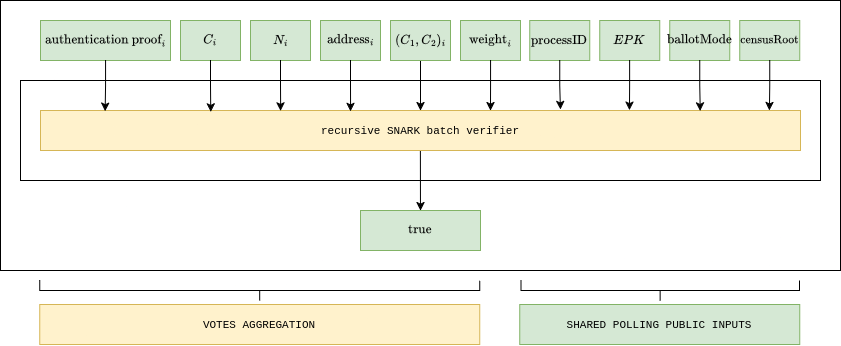
\includegraphics[width=400pt,draft=false]{\figs/circuit-aggregate}}
	\caption{Aggregation circuit. All public values are framed in green.}
	\label{fig:circuit-aggregate}
\end{figure}

\textbf{Inputs}:

\begin{itemize}
	\setlength\itemsep{1em}
	\item \public $\text{authenticationProof}$: set of authentication proofs.
	\item \public $C_i$: set of commitments.
	\item \public $N_i$: set of nullifiers.		
	\item \public $\address_i$: list of voters' addresses.
	\item \public $(C_1, C_2)$: list of voters' encrypted ballots.
	\item \public $\weight_i$: Voters' weights.
	\item \public $\processid$: process identifier.
	\item \public $EPK$: encryption public key.
	\item \public $\ballotmode$: ballot protocol configuration.
	\item \public $\text{censusRoot}$: census Merkle tree root.
\end{itemize}

\newpage
\subsubsection{State transition circuit}
